\documentclass[10pt,handout]{beamer}\usepackage[]{graphicx}\usepackage[]{color}
% maxwidth is the original width if it is less than linewidth
% otherwise use linewidth (to make sure the graphics do not exceed the margin)
\makeatletter
\def\maxwidth{ %
  \ifdim\Gin@nat@width>\linewidth
    \linewidth
  \else
    \Gin@nat@width
  \fi
}
\makeatother

\definecolor{fgcolor}{rgb}{0.345, 0.345, 0.345}
\newcommand{\hlnum}[1]{\textcolor[rgb]{0.686,0.059,0.569}{#1}}%
\newcommand{\hlstr}[1]{\textcolor[rgb]{0.192,0.494,0.8}{#1}}%
\newcommand{\hlcom}[1]{\textcolor[rgb]{0.678,0.584,0.686}{\textit{#1}}}%
\newcommand{\hlopt}[1]{\textcolor[rgb]{0,0,0}{#1}}%
\newcommand{\hlstd}[1]{\textcolor[rgb]{0.345,0.345,0.345}{#1}}%
\newcommand{\hlkwa}[1]{\textcolor[rgb]{0.161,0.373,0.58}{\textbf{#1}}}%
\newcommand{\hlkwb}[1]{\textcolor[rgb]{0.69,0.353,0.396}{#1}}%
\newcommand{\hlkwc}[1]{\textcolor[rgb]{0.333,0.667,0.333}{#1}}%
\newcommand{\hlkwd}[1]{\textcolor[rgb]{0.737,0.353,0.396}{\textbf{#1}}}%
\let\hlipl\hlkwb

\usepackage{framed}
\makeatletter
\newenvironment{kframe}{%
 \def\at@end@of@kframe{}%
 \ifinner\ifhmode%
  \def\at@end@of@kframe{\end{minipage}}%
  \begin{minipage}{\columnwidth}%
 \fi\fi%
 \def\FrameCommand##1{\hskip\@totalleftmargin \hskip-\fboxsep
 \colorbox{shadecolor}{##1}\hskip-\fboxsep
     % There is no \\@totalrightmargin, so:
     \hskip-\linewidth \hskip-\@totalleftmargin \hskip\columnwidth}%
 \MakeFramed {\advance\hsize-\width
   \@totalleftmargin\z@ \linewidth\hsize
   \@setminipage}}%
 {\par\unskip\endMakeFramed%
 \at@end@of@kframe}
\makeatother

\definecolor{shadecolor}{rgb}{.97, .97, .97}
\definecolor{messagecolor}{rgb}{0, 0, 0}
\definecolor{warningcolor}{rgb}{1, 0, 1}
\definecolor{errorcolor}{rgb}{1, 0, 0}
\newenvironment{knitrout}{}{} % an empty environment to be redefined in TeX

\usepackage{alltt}


%\usepackage{default}
\usepackage{animate} %need the animate.sty file 
\usepackage{graphicx}
%\graphicspath{{/home/sahir/Dropbox/jobs/laval/minicours/slides/}}
\usepackage{hyperref, url}
%\usepackage[round,sort]{natbib}   % bibliography omit 'round' option if you prefer square brackets
%\bibliographystyle{apalike}
\usepackage{biblatex}
\bibliography{bib.bib}
% Removes icon in bibliography
\setbeamertemplate{bibliography item}[text]

\usepackage[normalem]{ulem}

\setbeamertemplate{theorems}[numbered]

\setbeamertemplate{caption}[numbered]
\setbeamertemplate{caption label separator}{: }
\setbeamercolor{caption name}{fg=normal text.fg}

%\newtheorem{prop}{Proposition}
%\newenvironment{theoremc}[1]
%{\begin{shaded}\begin{theorem}[#1]}
%		{\end{theorem}\end{shaded}}
	
%\newtheorem{examplefirst}{Example}
%\newtheorem{examplesecond}{Example}
%\newenvironment<>{examplefirst}[1][]{%
%	\setbeamercolor{block title example}{bg=lightgray}%
%	\begin{example}#2[#1]}{\end{example}}
%\newenvironment<>{examplesecond}[1][]{%
%	\setbeamercolor{block title example}{fg=white,bg=blue!75!black}%
%	\begin{example}#2[#1]}{\end{example}}	

%\usepackage{amsthm}


\usepackage[figurename=Fig.]{caption}
\usepackage{subfig}
\usepackage{tikz, pgfplots,epsfig}
\usetikzlibrary{arrows,shapes.geometric}
\usepackage{color, colortbl,xcolor}
\definecolor{lightgray}{RGB}{200,200,200}
\definecolor{palegray}{RGB}{221,221,221}
\definecolor{myblue}{RGB}{0,89,179}
\definecolor{myorange}{rgb}{0.776,0.357,0.157}

\definecolor{gray}{RGB}{110,110,110}
\definecolor{darkgray}{RGB}{100,100,100}
\definecolor{lightgray}{RGB}{200,200,200}
\definecolor{turquoise}{RGB}{81,193,188}
\definecolor{tomato}{RGB}{255,136,136}
\definecolor{mandarina}{RGB}{229,169,25}
\definecolor{foreground}{RGB}{81,141,193}
\definecolor{background}{RGB}{246,244,240}
\definecolor{highlight}{RGB}{229,169,25}
\definecolor{lowlight}{RGB}{200,200,200}
\definecolor{beige}{RGB}{255,255,240}
\definecolor{pinkish}{RGB}{255,223,247}

\newcommand{\code}[1]{\texttt{#1}}


\usepackage{comment}
\setbeamercolor{frametitle}{fg=myblue}
\setbeamercolor{section in head/foot}{bg=myblue, fg=white}
\setbeamercolor{author in head/foot}{bg=myblue}
\setbeamercolor{date in head/foot}{bg=myblue}

\usepackage{amsthm}
\usepackage{shadethm}
%\colorlet{shadecolor}{blue!15}
\colorlet{shadecolor}{palegray}
%\setlength{\shadeboxrule}{.4pt}

%\newshadetheorem{thm}{Theorem}
\newshadetheorem{defm}{Definition}
\newshadetheorem{exm}{Exercise}
\newshadetheorem{remarkm}{Remark}
%\definecolor{shadethmcolor}{HTML}{EDF8FF}
\definecolor{shadethmcolor}{RGB}{221,221,221}
%\definecolor{shaderulecolor}{HTML}{45CFFF}
\definecolor{shaderulecolor}{RGB}{0,89,179}
\setlength{\shadeboxrule}{.4pt}

\newtheorem{thm}{Theorem}
\newcommand{\statetheoremhoriz}[2][\textwidth]{
	\par\noindent\tikzstyle{mybox} = [draw=myblue,left color=cyan!50,
	right color=cyan!5,thick,rectangle,inner sep=6pt]
	\begin{tikzpicture}
	\node [mybox] (box){%
		\begin{minipage}{#1}{#2}\end{minipage}
	};
	\end{tikzpicture}
}
\newcommand{\statetheoremvert}[2][\textwidth]{
	\par\noindent\tikzstyle{mybox} = [draw=myblue,top color=cyan!50,
	bottom color=cyan!5,thick,rectangle,inner sep=6pt]
	\begin{tikzpicture}
	\node [mybox] (box){%
		\begin{minipage}{#1}{#2}\end{minipage}
	};
	\end{tikzpicture}
}
\newcommand{\statetheoremsolid}[2][\textwidth]{
	\par\noindent\tikzstyle{mybox} = [draw=myblue,fill=palegray,
	thick,rectangle,inner sep=6pt]
	\begin{tikzpicture}
	\node [mybox] (box){%
		\begin{minipage}{#1}{#2}\end{minipage}
	};
	\end{tikzpicture}
}

\usetikzlibrary{shapes.geometric, arrows,shapes.symbols,decorations.pathreplacing}
\tikzstyle{startstop} = [rectangle, rounded corners, minimum width=3cm, minimum height=1cm, draw=black, fill=pinkish,text width=3.5cm]
\tikzstyle{startstop2} = [rectangle, rounded corners, minimum width=3cm, minimum height=1cm, draw=black, fill=background,text width=4.5cm]
\tikzstyle{startstop3} = [rectangle, rounded corners, minimum width=3cm, minimum height=1cm, draw=black, fill=beige,text width=3.0cm]
\tikzstyle{startstop4} = [rectangle, rounded corners, minimum width=3cm, minimum height=1cm, draw=black, fill=pinkish,text width=4.5cm]
\tikzstyle{io} = [trapezium, trapezium left angle=70, trapezium right angle=110, minimum width=2cm, minimum height=1cm, text centered, draw=black, fill=blue!30,text width=1.5cm]
\tikzstyle{process} = [rectangle, minimum width=1cm, minimum height=1cm, text centered, draw=black, fill=orange!30,text width=2cm]
\tikzstyle{decision} = [diamond, minimum width=2cm, minimum height=1cm, text centered, draw=black, fill=green!30]
\tikzstyle{arrow} = [thick,->,>=stealth]
\tikzstyle{both} = [thick,<->,>=stealth, red]


\usepackage{array}
\newcolumntype{L}{>{\centering\arraybackslash}m{3cm}} % used for text wrapping in ctable
\usepackage{ctable}
\usepackage[utf8]{inputenc}
\usepackage{fontenc}
\usepackage{pifont}% http://ctan.org/pkg/pifont
\newcommand{\cmark}{\ding{51}}%
\newcommand{\xmark}{\ding{55}}%
\def\widebar#1{\overline{#1}}
\definecolor{whitesmoke}{rgb}{0.96, 0.96, 0.96}

\usepackage{amssymb}
\usepackage{amsmath}

\usepackage{bm}
\def\transpose{{\sf{T}}}
\def\E{{\skew0\bm{E}}}
\def\Xvec{{\skew0\bm{X}}}
\def\Xveca{{\skew0\bm{X}}_1}
\def\Xvecb{{\skew0\bm{X}}_2}

\def\Yvec{{\skew0\bm{Y}}}
\def\bmY{{\skew0\bm{Y}}}
\def\bmX{{\skew0\bm{X}}}
\def\bmy{{\skew0\bm{y}}}
\def\bmG{{\skew0\bm{G}}}
\def\bmS{{\skew0\bm{S}}}
\def\bmA{{\skew0\bm{A}}}
\def\bmB{{\skew0\bm{B}}}
\def\bmD{{\skew0\bm{D}}}
\def\bmI{{\skew0\bm{I}}}
\def\bmV{{\skew0\bm{V}}}
\def\bmU{{\skew0\bm{U}}}
\def\bv{{\skew0\bm{v}}}
\def\bw{{\skew0\bm{w}}}
\def\bmm{{\skew0\bm{m}}}
\def\bmzero{{\skew0\bm{0}}}
\def\bx{{\skew0\bm{x}}}
\def\xveca{{\skew0\bm{x}}_1}
\def\xvecb{{\skew0\bm{x}}_2}

\def\N{{\skew0\mathcal{N}}}
\def\T{{\small T}}

\def\mvec{{\skew0\bm{m}}}
\def\bmmu{{\skew0\bm{\mu}}}
\def\muvec{{\skew0\bm{\mu}}}
\def\balpha{{\skew0\bm{\alpha}}}
\def\bbeta{{\skew0\bm{\beta}}}
\def\bmtheta{{\skew0\bm{\theta}}}
\def\btheta{{\skew0\bm{\theta}}}

\def\cvec{{\skew0\mathbf{c}}}

\def\Xbar{\overline{X}}

\definecolor{lightgray}{rgb}{0.91,0.91,0.91}
\definecolor{purpleblue}{rgb}{0.50,0.50,1.00}



\usepackage{fontspec}
%\setsansfont{Fira Sans}
%\setmonofont{Fira Mono}
%\setsansfont[ItalicFont={Fira Sans Light Italic},BoldFont={Fira Sans},BoldItalicFont={Fira Sans Italic}]{Fira Sans Light}
%\setmonofont[BoldFont={Fira Mono Medium}]{Fira Mono}

\def\installpath{/usr/local/share/texmf/fonts/opentype/libertinus/}
\setmainfont{LibertinusSerif}[
UprightFont    = *-Regular,
BoldFont       = *-Bold,
ItalicFont     = *-Italic,
BoldItalicFont = *-BoldItalic,
Ligatures      = TeX,
Extension      = .otf,
Path           = \installpath/
]

\setsansfont{LibertinusSerif}[
UprightFont    = *-Regular,
BoldFont       = *-Bold,
ItalicFont     = *-Italic,
BoldItalicFont = *-BoldItalic,
Ligatures      = TeX,
Extension      = .otf,
Path           = \installpath/
]


\setmonofont{LibertinusSerif}[
UprightFont    = *-Regular,
BoldFont       = *-Bold,
ItalicFont     = *-Italic,
BoldItalicFont = *-BoldItalic,
Ligatures      = TeX,
Extension      = .otf,
Path           = \installpath/
]



\setbeamercolor{itemize item}{fg=myblue}
%\setbeamertemplate{itemize item}[square]
\setbeamertemplate{itemize items}[circle]
%\setbeamertemplate{blocks}[rounded][shadow=true]


%\setbeamertemplate{navigation symbols}{\usebeamercolor[fg]{title in head/foot}\usebeamerfont{title in head/foot}\insertframenumber}


%\setbeamertemplate{footline}{}

\beamertemplatenavigationsymbolsempty % toggle off if you want navigation symbols at the bottom

\setbeamertemplate{footline}
{ \usebeamercolor[fg]{page number in head/foot}%
	\usebeamerfont{page number in head/foot}%
	\hspace{1em}\insertsectionhead%
	\hfill%
	\insertframenumber\,/\,\hyperlinkappendixstart{\insertmainframenumber}
	\ifnum \thepage = \insertframeendpage{\small .}\else{\phantom{\small .}}\fi
	\hspace{1em}
	\vskip2pt%
}

\newtheorem{proposition}[theorem]{Proposition}
\newtheorem{exercise}[theorem]{Exercise}

\titlegraphic{\hfill
\includegraphics[height=1cm]{../mcgill_logo.png}}


%% You also use hyperref, and pick colors 
\hypersetup{colorlinks,citecolor=myorange,filecolor=red,linkcolor=brown,urlcolor=blue}

\newcommand {\framedgraphiccaption}[2] {
	\begin{figure}
		\centering
		\includegraphics[width=\textwidth,height=0.8\textheight,keepaspectratio]{#1}
		\caption{#2}
	\end{figure}
}

\newcommand {\framedgraphic}[1] {
	\begin{figure}
		\centering
		\includegraphics[width=\textwidth,height=0.9\textheight,keepaspectratio]{#1}
	\end{figure}
}


\AtBeginSection[]{
	\begin{frame}
		\vfill
		\centering
		\begin{beamercolorbox}[sep=8pt,center,shadow=true,rounded=true]{title}
			\usebeamerfont{title}\insertsectionhead\par%
		\end{beamercolorbox}
		\vfill
	\end{frame}
}

\newcommand\Wider[2][3em]{%
	\makebox[\linewidth][c]{%
		\begin{minipage}{\dimexpr\textwidth+#1\relax}
			\raggedright#2
		\end{minipage}%
	}%
}


\makeatletter

\def \iqsssectiontitleheader {}

\newcommand{\iqsssectiontitle}[1]{
	\def \iqsssectiontitleheader{#1}
}

\@ifundefined{insertmainframenumber}
{%
	% \insertmainframenumber not defined
	\newcommand{\insertmainframenumber}{\inserttotalframenumber}
}
{%
	% \insertmainframenumber already defined
}%


\AtBeginSection[]{
	\title{\insertsectionhead}
	{
		%\definecolor{white}{RGB}{140,193,250}
		%\definecolor{white}{RGB}{200,200,200}
		%\definecolor{white}{RGB}{242,244,247}
		\definecolor{white}{RGB}{0,89,179}
		%\definecolor{iqss@orange}{rgb}{1,1,1}
		\ifnum \insertmainframenumber > \insertframenumber
		%\setbeamercolor{background canvas}{bg=myblue}
		%\setbeamercolor{normal text}{fg=black,bg=white}
		%\setbeamercolor{frametitle}{fg=red}
		%\setbeamercolor{section in toc}{fg=myblue, bg=white}
		%\setbeamercolor{subsection in toc}{fg=myblue, bg=white}
		\frame{
			\frametitle{\iqsssectiontitleheader}
			\tableofcontents[currentsection]
		}
		\else
		\frame{
			\frametitle{Backup Slides}
			\tableofcontents[sectionstyle=shaded/shaded,subsectionstyle=shaded/shaded/shaded]
		}
		\fi
	}
}
\makeatother

\pgfplotsset{compat=1.16}
\usepackage{graphicx}
\usepackage{hyperref, url}
\hypersetup{colorlinks,citecolor=myorange,filecolor=red,linkcolor=brown,urlcolor=blue}

\usepackage{longtable,booktabs}

\usepackage{subfig}
\usepackage{tikz}
\usetikzlibrary{shapes.geometric, arrows,shapes.symbols,decorations.pathreplacing}
\tikzstyle{startstop} = [rectangle, rounded corners, minimum width=3cm, minimum height=1cm, draw=black, fill=pinkish,text width=3.5cm]
\tikzstyle{startstop2} = [rectangle, rounded corners, minimum width=3cm, minimum height=1cm, draw=black, fill=background,text width=4.5cm]
\tikzstyle{startstop3} = [rectangle, rounded corners, minimum width=3cm, minimum height=1cm, draw=black, fill=beige,text width=3.0cm]
\tikzstyle{startstop4} = [rectangle, rounded corners, minimum width=3cm, minimum height=1cm, draw=black, fill=pinkish,text width=4.5cm]
\tikzstyle{io} = [trapezium, trapezium left angle=70, trapezium right angle=110, minimum width=2cm, minimum height=1cm, text centered, draw=black, fill=blue!30,text width=1.5cm]
\tikzstyle{process} = [rectangle, minimum width=1cm, minimum height=1cm, text centered, draw=black, fill=orange!30,text width=2cm]
\tikzstyle{decision} = [diamond, minimum width=2cm, minimum height=1cm, text centered, draw=black, fill=green!30]
\tikzstyle{arrow} = [thick,->,>=stealth]
\tikzstyle{both} = [thick,<->,>=stealth, red]


% used for tree of stats tests in 001-introduction
\tikzstyle{startstopstats} = [rectangle, rounded corners, minimum width=2cm, minimum height=.5cm,text centered, draw=black, fill=red!30]
\tikzstyle{iostats} = [trapezium, trapezium left angle=70, trapezium right angle=110, minimum width=2cm, minimum height=.5cm, text centered, draw=black, fill=blue!30]
\tikzstyle{processstats} = [rectangle, minimum width=1.5cm, minimum height=.5cm, text centered, draw=black, fill=orange!30]
\tikzstyle{processbigstats} = [rectangle, minimum width=1.5cm, minimum height=.5cm, text centered, draw=black, fill=orange!30,text width=1.6cm]
\tikzstyle{decisionstats} = [rectangle, minimum width=1cm, minimum height=1cm, text centered, draw=black, fill=green!30,text width=1.6cm]
\tikzstyle{decisionbigstats} = [rectangle, minimum width=1cm, minimum height=1cm, text centered, draw=black, fill=yellow!30,text width=2cm]





\usepackage{color, colortbl,xcolor}
\definecolor{lightgray}{RGB}{200,200,200}
\definecolor{palegray}{RGB}{221,221,221}
\definecolor{myblue}{RGB}{0,89,179}
\definecolor{myorange}{rgb}{0.776,0.357,0.157}
\definecolor{gray}{RGB}{110,110,110}
\definecolor{darkgray}{RGB}{100,100,100}
\definecolor{lightgray}{RGB}{200,200,200}
\definecolor{turquoise}{RGB}{81,193,188}
\definecolor{tomato}{RGB}{255,136,136}
\definecolor{mandarina}{RGB}{229,169,25}
\definecolor{foreground}{RGB}{81,141,193}
\definecolor{background}{RGB}{246,244,240}
\definecolor{highlight}{RGB}{229,169,25}
\definecolor{lowlight}{RGB}{200,200,200}
\definecolor{beige}{RGB}{255,255,240}
\definecolor{pinkish}{RGB}{255,223,247}

\newcommand{\code}[1]{\texttt{#1}}


\usepackage{comment}

\makeatletter

\def \iqsssectiontitleheader {}

\newcommand{\iqsssectiontitle}[1]{
	\def \iqsssectiontitleheader{#1}
}

\@ifundefined{insertmainframenumber}
{%
	% \insertmainframenumber not defined
	\newcommand{\insertmainframenumber}{\inserttotalframenumber}
}
{%
	% \insertmainframenumber already defined
}%


\AtBeginSection[]{
	\title{\insertsectionhead}
	{
		%\definecolor{white}{RGB}{140,193,250}
		%\definecolor{white}{RGB}{200,200,200}
		%\definecolor{white}{RGB}{242,244,247}
		\definecolor{white}{RGB}{0,89,179}
		%\definecolor{iqss@orange}{rgb}{1,1,1}
		\ifnum \insertmainframenumber > \insertframenumber
		%\setbeamercolor{background canvas}{bg=myblue}
		%\setbeamercolor{normal text}{fg=black,bg=white}
		%\setbeamercolor{frametitle}{fg=red}
		%\setbeamercolor{section in toc}{fg=myblue, bg=white}
		%\setbeamercolor{subsection in toc}{fg=myblue, bg=white}
		\frame{
			\frametitle{\iqsssectiontitleheader}
			\tableofcontents[currentsection]
		}
		\else
		\frame{
			\frametitle{Backup Slides}
			\tableofcontents[sectionstyle=shaded/shaded,subsectionstyle=shaded/shaded/shaded]
		}
		\fi
	}
}
\makeatother
%\graphicspath{{/home/sahir/git_repositories/EPIB607/resources/assets/slides/figure/}}


\usepackage{fontspec}
%\setsansfont{Fira Sans}
%\setmonofont{Fira Mono}
%\setsansfont[ItalicFont={Fira Sans Light Italic},BoldFont={Fira Sans},BoldItalicFont={Fira Sans Italic}]{Fira Sans Light}
%\setmonofont[BoldFont={Fira Mono Medium}]{Fira Mono}

\def\installpath{/usr/local/share/texmf/fonts/opentype/libertinus/}
\setmainfont{LibertinusSerif}[
UprightFont    = *-Regular,
BoldFont       = *-Bold,
ItalicFont     = *-Italic,
BoldItalicFont = *-BoldItalic,
Ligatures      = TeX,
Extension      = .otf,
Path           = \installpath/
]

\setsansfont{LibertinusSerif}[
UprightFont    = *-Regular,
BoldFont       = *-Bold,
ItalicFont     = *-Italic,
BoldItalicFont = *-BoldItalic,
Ligatures      = TeX,
Extension      = .otf,
Path           = \installpath/
]


%\setmonofont{LibertinusSerif}[
%UprightFont    = *-Regular,
%BoldFont       = *-Bold,
%ItalicFont     = *-Italic,
%BoldItalicFont = *-BoldItalic,
%Ligatures      = TeX,
%Extension      = .otf,
%Path           = \installpath/
%]






\newcommand\Wider[2][3em]{%
	\makebox[\linewidth][c]{%
		\begin{minipage}{\dimexpr\textwidth+#1\relax}
			\raggedright#2
		\end{minipage}%
	}%
}


\newcommand {\framedgraphic}[1] {
	\begin{figure}
		\centering
		\includegraphics[width=\textwidth,height=0.9\textheight,keepaspectratio]{#1}
	\end{figure}
}


\setbeamercolor{itemize item}{fg=myblue}
\setbeamercolor{itemize subitem}{fg=myorange}
%\setbeamertemplate{itemize item}[square]
\setbeamertemplate{itemize item}[circle]
\setbeamertemplate{itemize subitem}[triangle]
%\setbeamertemplate{blocks}[rounded][shadow=true]


%\setbeamertemplate{navigation symbols}{\usebeamercolor[fg]{title in head/foot}\usebeamerfont{title in head/foot}\insertframenumber}


%\setbeamertemplate{footline}{}

\beamertemplatenavigationsymbolsempty % toggle off if you want navigation symbols at the bottom

\setbeamertemplate{footline}
{ \usebeamercolor[fg]{page number in head/foot}%
	\usebeamerfont{page number in head/foot}%
	\hspace{1em}\insertsectionhead%
	\hfill%
	\insertframenumber\,/\,\hyperlinkappendixstart{\insertmainframenumber}
	\ifnum \thepage = \insertframeendpage{\small .}\else{\phantom{\small .}}\fi
	\hspace{1em}
	\vskip2pt%
}

\newtheorem{proposition}[theorem]{Proposition}
\newtheorem{exercise}[theorem]{Exercise}



\setlength{\emergencystretch}{3em} % prevent overfull lines
\providecommand{\tightlist}{%
	\setlength{\itemsep}{0pt}\setlength{\parskip}{0pt}}




\titlegraphic{\hfill
\includegraphics[height=1cm]{/home/sahir/git_repositories/EPIB607/resources/assets/slides/mcgill_logo.png}}
\graphicspath{{/home/sahir/git_repositories/EPIB607/resources/assets/slides/figure/}}

%\let\oldShaded\Shaded
%\let\endoldShaded\endShaded
%\renewenvironment{Shaded}{\footnotesize\oldShaded}{\endoldShaded}
\IfFileExists{upquote.sty}{\usepackage{upquote}}{}
\begin{document}
	
	
	
	%\title{Introduction to Regression Trees}
	%\author{Sahir Bhatnagar \inst{1}}
	%\author[shortname]{Sahir Rai Bhatnagar, PhD Candidate (Biostatistics) }
	%\institute[shortinst]{Department of Epidemiology, Biostatistics and Occupational Health}
	
	\title{004 - Exploring Data - Part II}
	\author{EPIB 607 - FALL 2020}
	\institute{
		Sahir Rai Bhatnagar\\
		Department of Epidemiology, Biostatistics, and Occupational Health\\
		McGill University\\
		
		\vspace{0.1 in}
		
		\texttt{sahir.bhatnagar@mcgill.ca}\\
		%\texttt{\url{https://sahirbhatnagar.com/EPIB607/}}
	}
	
	\date{slides compiled on \today}
	
	\maketitle

	
	

						
\begin{frame}{Summarizing relationships between two variables}
							\protect\hypertarget{summarizing-relationships-between-two-variables}{}
							
							Approaches for summarizing relationships between two variables vary
							depending on variable types:
							
							\begin{itemize}
								\item
								Two numerical variables
								\item
								Two categorical variables
								\item
								One numerical variable and one categorical variable
							\end{itemize}
							
\end{frame}


\section{Two numerical variables}


\begin{frame}[fragile]{Scatterplots}
	\protect\hypertarget{two-numerical-variables-1}{}
	
	\small
	
	\scriptsize
	
	
\begin{knitrout}\scriptsize
\definecolor{shadecolor}{rgb}{0.969, 0.969, 0.969}\color{fgcolor}\begin{kframe}
\begin{alltt}
\hlkwd{library}\hlstd{(ggplot2);} \hlkwd{library}\hlstd{(oibiostat);}
\hlkwd{data}\hlstd{(famuss)}

\hlkwd{plot}\hlstd{(famuss}\hlopt{$}\hlstd{height, famuss}\hlopt{$}\hlstd{weight,} \hlkwc{xlab} \hlstd{=} \hlstr{"Height (in)"}\hlstd{,} \hlkwc{ylab} \hlstd{=} \hlstr{"Weight (lb)"}\hlstd{)}

\hlkwd{ggplot}\hlstd{(}\hlkwc{data} \hlstd{= famuss,} \hlkwc{mapping} \hlstd{=} \hlkwd{aes}\hlstd{(}\hlkwc{x} \hlstd{= height,} \hlkwc{y} \hlstd{= weight))} \hlopt{+}
  \hlkwd{geom_point}\hlstd{(}\hlkwc{size} \hlstd{=} \hlnum{0.8}\hlstd{,} \hlkwc{pch} \hlstd{=} \hlnum{21}\hlstd{)}
\end{alltt}
\end{kframe}

{\centering 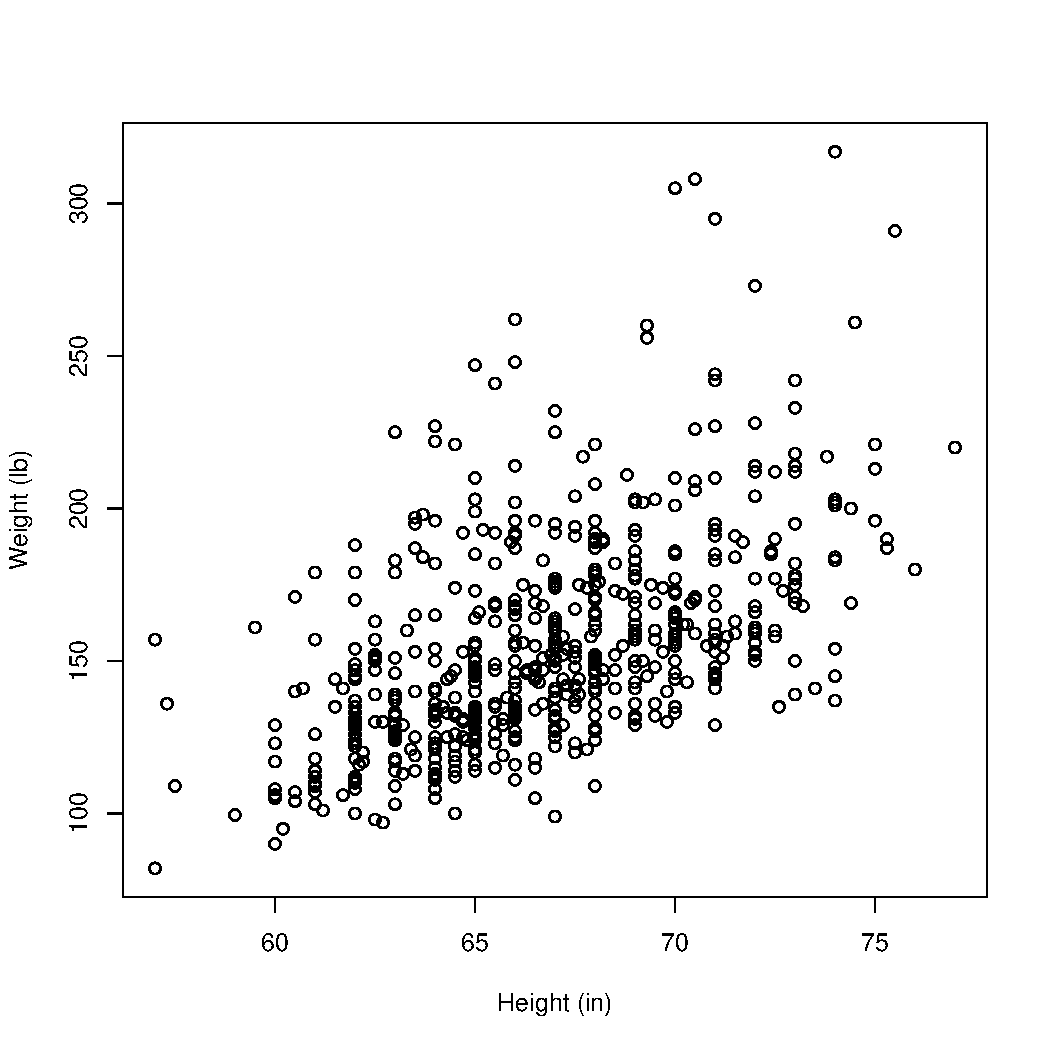
\includegraphics[width=0.45\linewidth]{figure/numerical-1} 
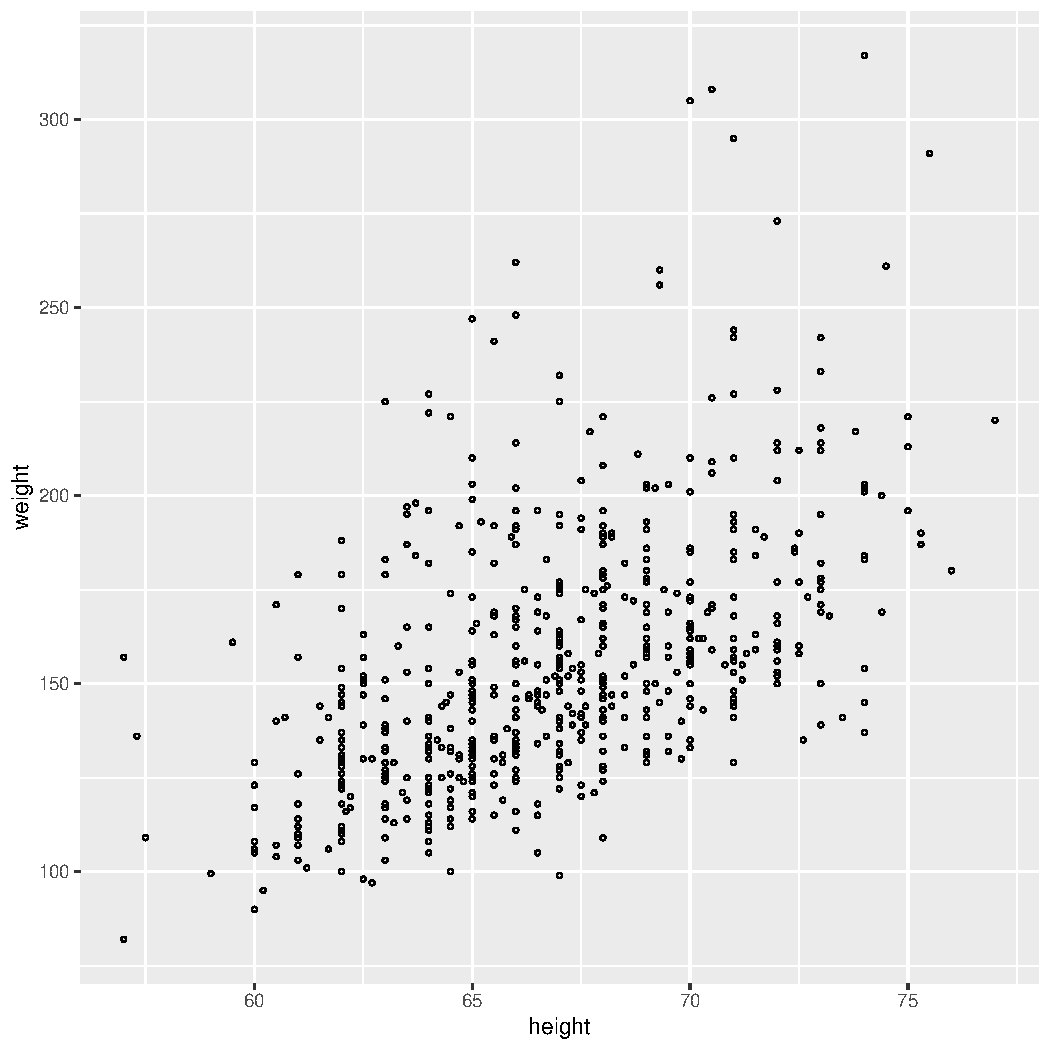
\includegraphics[width=0.45\linewidth]{figure/numerical-2} 

}



\end{knitrout}
	
	\normalsize
	
\end{frame}



						
						\begin{frame}{Correlation coefficient}
							\protect\hypertarget{two-numerical-variables}{}
							
								\begin{itemize}
							
							\item The correlation between two variables $x$ and $y$ is given by:
							$$
							r=\frac{1}{n-1} \sum_{i=1}^{n}\left(\frac{x_{i}-\bar{x}}{s_{x}}\right)\left(\frac{y_{i}-\bar{y}}{s_{y}}\right)
							$$
							where $\left(x_{1}, y_{1}\right),\left(x_{2}, y_{2}\right), \ldots,\left(x_{n}, y_{n}\right)$ are the $n$ paired values of $x$ and $y,$ and $s_{x}$ and $s_{y}$ are the sample standard deviations of the $x$ and $y$ variables, respectively.
							
							
							\pause 
							
							\item The correlation coefficient quantifies the strength of a \textbf{\textcolor{red}{linear}} trend.
							
							\pause
							
								\item
							The correlation coefficient \(r\) takes on values between -1 and 1.
							\pause 
							\item
							The closer \(r\) is to \(\pm 1\), the stronger the linear association.
							\pause 
							
\item 	Two variables \(x\) and \(y\) are
							
							\begin{itemize}
								\item
								\emph{positively associated} if \(y\) increases as \(x\) increases ($r>0$)
								\item
								\emph{negatively associated} if \(y\) decreases as \(x\) increases ($r<0$)
							\end{itemize}
						
													\end{itemize}
							
							
						\end{frame}
						


						
\begin{frame}[fragile]{Correlation in \texttt{R}}
							\protect\hypertarget{two-numerical-variables-2}{}

							\begin{itemize}							
		\item Correlation between weight and height in the \texttt{famuss} dataset:
							
						
						
\begin{knitrout}\scriptsize
\definecolor{shadecolor}{rgb}{0.969, 0.969, 0.969}\color{fgcolor}\begin{kframe}
\begin{alltt}
\hlkwd{cor}\hlstd{(famuss}\hlopt{$}\hlstd{height, famuss}\hlopt{$}\hlstd{weight)}
\end{alltt}
\begin{verbatim}
## [1] 0.53
\end{verbatim}
\end{kframe}
\end{knitrout}
							
							\pause
							
							\item We can also obtain the correlation between \texttt{weight} and \texttt{height} from a simple linear regression:
							
\begin{knitrout}\scriptsize
\definecolor{shadecolor}{rgb}{0.969, 0.969, 0.969}\color{fgcolor}\begin{kframe}
\begin{alltt}
\hlkwd{summary}\hlstd{(}\hlkwd{lm}\hlstd{(height} \hlopt{~} \hlstd{weight,} \hlkwc{data} \hlstd{= famuss))}
\end{alltt}
\begin{verbatim}
## Coefficients:
##             Estimate Std. Error t value Pr(>|t|)    
## (Intercept)  58.2952     0.5732   101.7   <2e-16 ***
## weight        0.0548     0.0036    15.2   <2e-16 ***
## ---
## Signif. codes:  0 '***' 0.001 '**' 0.01 '*' 0.05 '.' 0.1 ' ' 1
## 
## Residual standard error: 3 on 593 degrees of freedom
## Multiple R-squared: 0.282,	Adjusted R-squared: 0.281 
## F-statistic:  233 on 1 and 593 DF,  p-value: <2e-16
\end{verbatim}
\end{kframe}
\end{knitrout}
						
							\normalsize
							
					\end{itemize}
							
						\end{frame}




\begin{frame}{Another example: NHANES\footnote{\tiny{\url{http://www.cdc.gov/nchs/nhanes.htm}}}}
	\begin{itemize}
		\item The National Health and Nutrition Examination Survey (NHANES) consists of a set of surveys and measurements conducted by the US CDC to assess the health and nutritional status of adults	and children in the United States. 
		\item The following example uses data from a sample of 500 adults (individuals ages 21 and older) from the NHANES dataset\footnote{\tiny{The sample is available as \texttt{nhanes.samp.adult.500} in the \texttt{R} \code{oibiostat} package}}.
	\end{itemize}
\end{frame}

\begin{frame}[fragile,plain]

\vspace{-0.5in}	
	
\begin{knitrout}\tiny
\definecolor{shadecolor}{rgb}{0.969, 0.969, 0.969}\color{fgcolor}\begin{figure}

{\centering \subfloat[\label{fig:unnamed-chunk-1-1}]{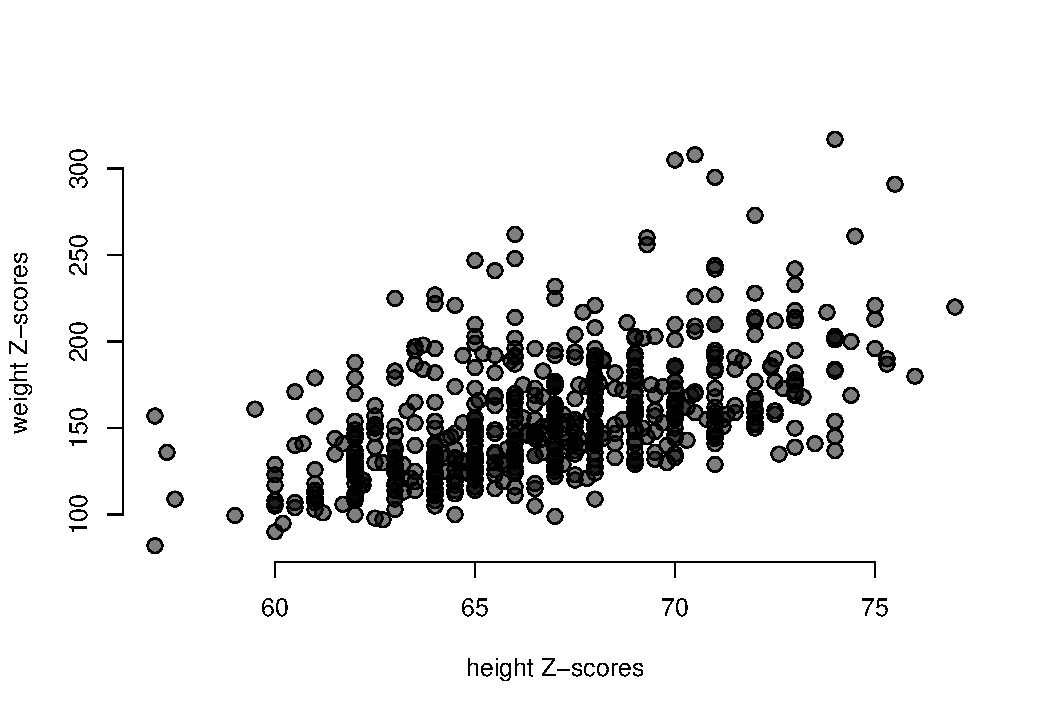
\includegraphics[width=0.55\linewidth]{figure/unnamed-chunk-1-1} }
\subfloat[\label{fig:unnamed-chunk-1-2}]{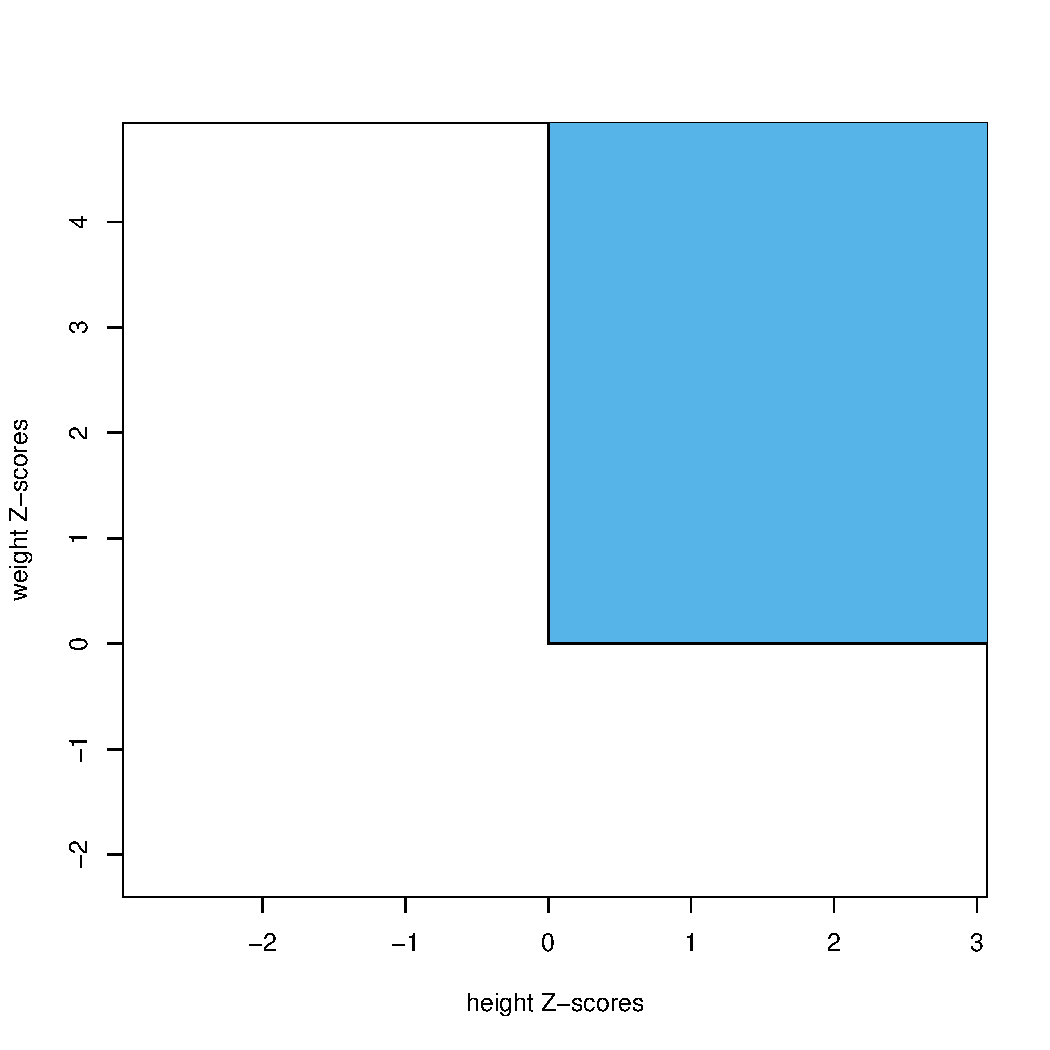
\includegraphics[width=0.55\linewidth]{figure/unnamed-chunk-1-2} }

}

\caption[(a) A scatterplot showing height versus weight from the 500 individuals in the sample from NHANES]{(a) A scatterplot showing height versus weight from the 500 individuals in the sample from NHANES. One participant 163.9 cm tall (about 5 ft, 4 in) and weighing 144.6 kg (about 319 lb) is highlighted. (b) A scatterplot showing height versus BMI from the 500 individuals in the sample from NHANES. The same individual highlighted in (a) is marked here, with BMI 53.83. Fitted regression lines are shown in red with correlation coefficient $r$. BMI = weight/height$^2$ $\times 703$.}\label{fig:unnamed-chunk-1}
\end{figure}


\end{knitrout}
	
\end{frame}










\begin{frame}[fragile]{Anscombe's quartet\footnote{\tiny{Anscombe, Francis J. (1973). Graphs in statistical analysis. The American Statistician, 27, 17–21. doi: 10.2307/2682899.}}}
	
\begin{knitrout}\tiny
\definecolor{shadecolor}{rgb}{0.969, 0.969, 0.969}\color{fgcolor}\begin{kframe}
\begin{alltt}
\hlkwd{library}\hlstd{(datasets);}\hlkwd{data}\hlstd{(}\hlstr{"anscombe"}\hlstd{)}
\end{alltt}
\end{kframe}\begin{figure}

{\centering 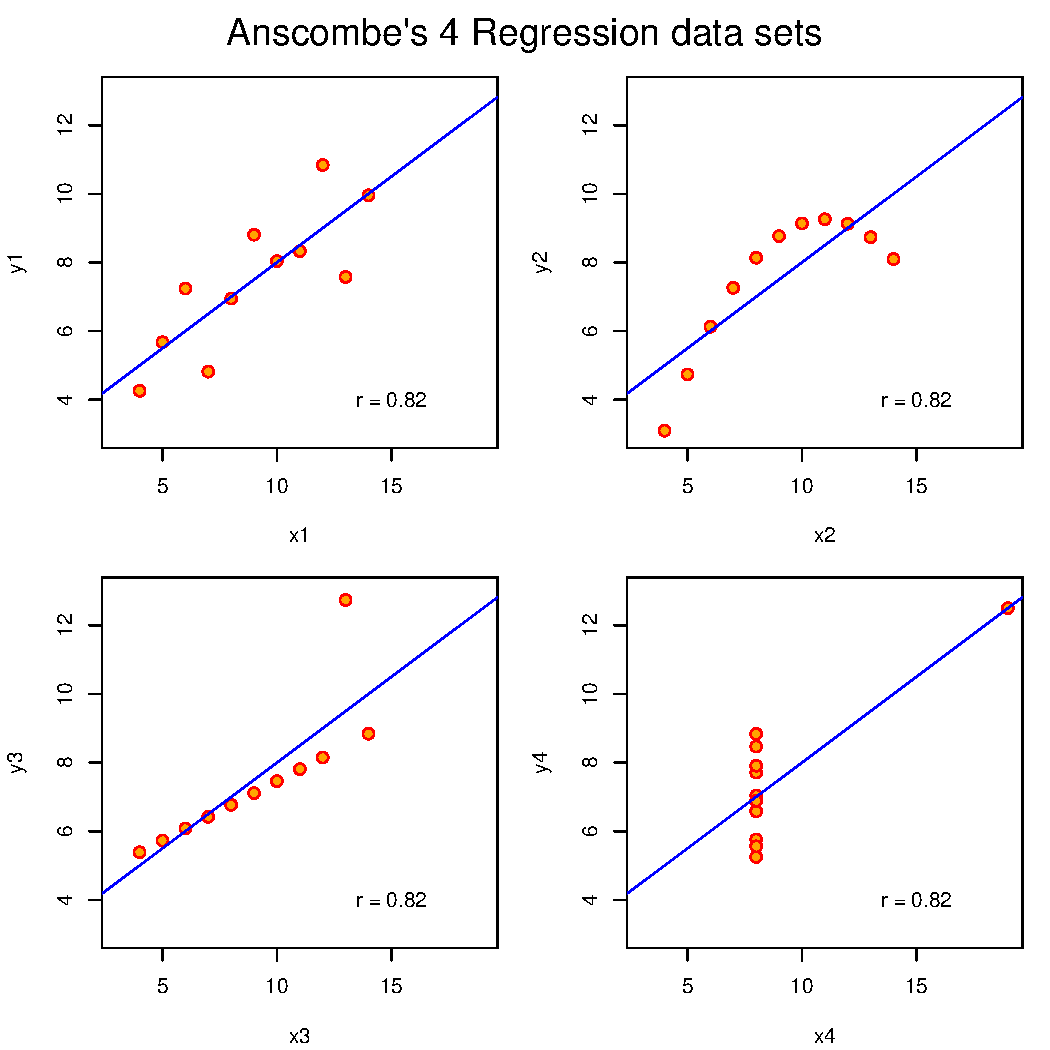
\includegraphics[width=0.55\linewidth]{figure/unnamed-chunk-2-1} 

}

\caption[All four panels have the exact same linear correlation coefficient]{All four panels have the exact same linear correlation coefficient}\label{fig:unnamed-chunk-2}
\end{figure}


\end{knitrout}


\end{frame}





\begin{frame}[fragile,plain]
	
\begin{knitrout}\tiny
\definecolor{shadecolor}{rgb}{0.969, 0.969, 0.969}\color{fgcolor}\begin{figure}

{\centering \subfloat[\label{fig:004-nyt-1}]{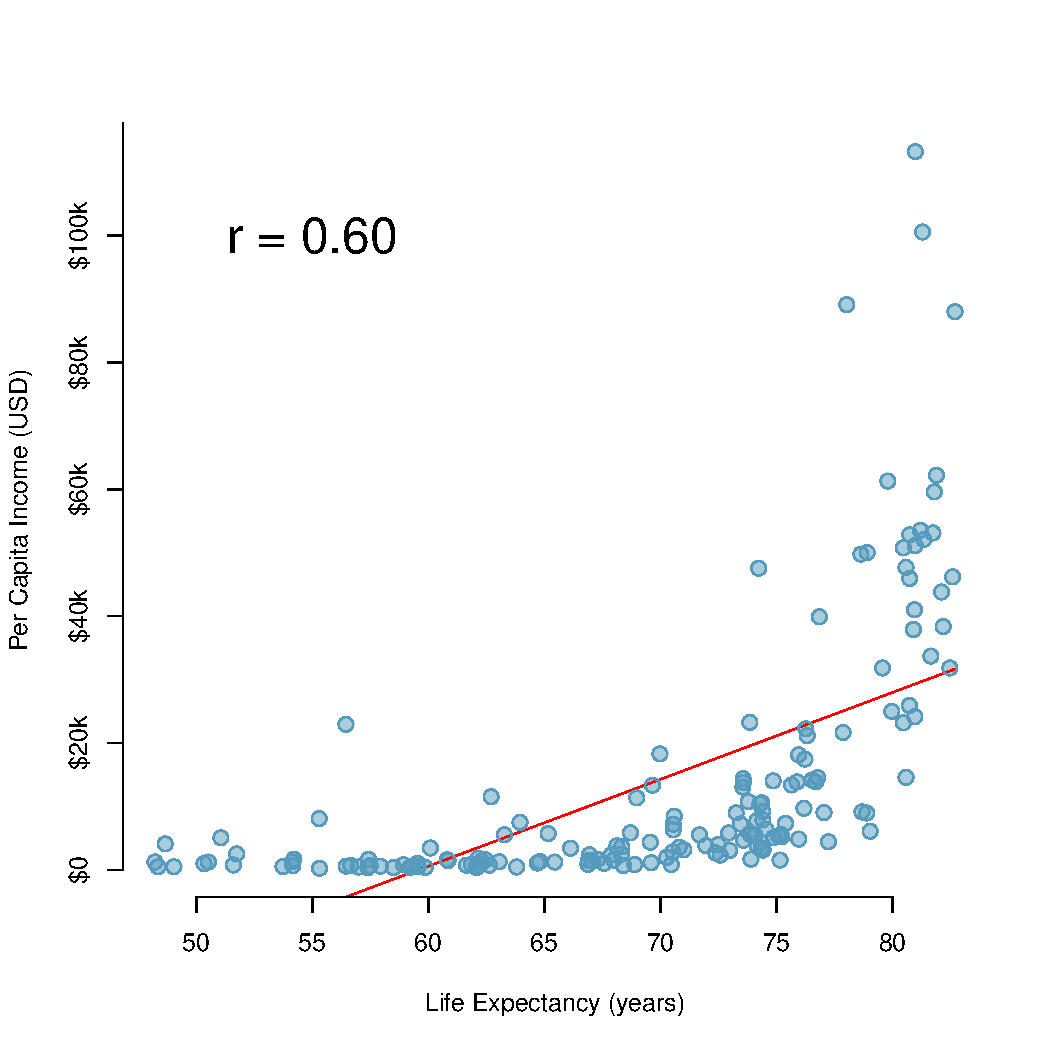
\includegraphics[width=0.53\linewidth]{figure/004-nyt-1} }
\subfloat[\label{fig:004-nyt-2}]{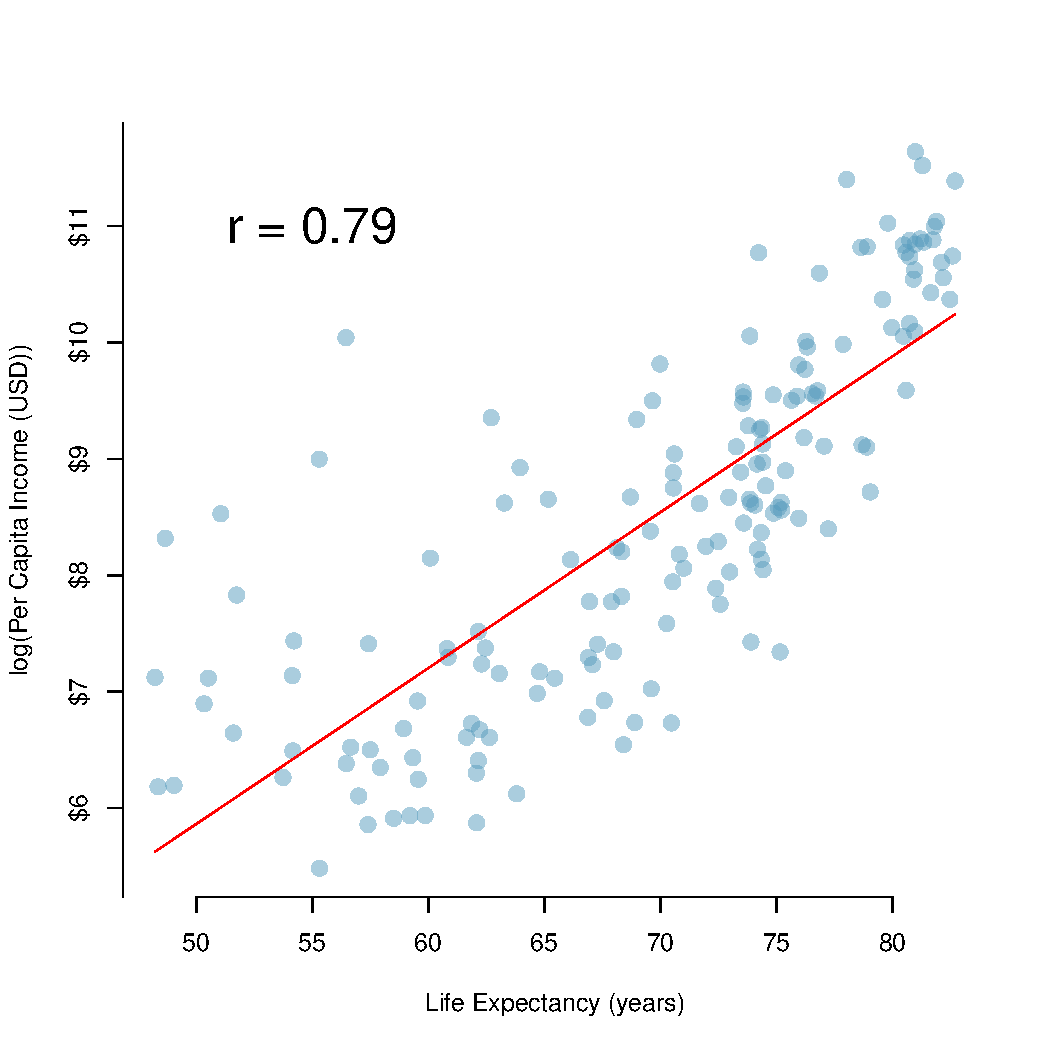
\includegraphics[width=0.53\linewidth]{figure/004-nyt-2} }

}

\caption{(a) per capita income vs. life expectancy (b) log per capita income vs. life expectancy. Fitted regression line in red with correlation coefficient $r$.\footnote{\tiny{The World Development Indicators (WDI) is a database of country-level variables (i.e., indicators) recording outcomes for a variety of topics, including economics, health, mortality, fertility, and education}}}\label{fig:004-nyt}
\end{figure}


\end{knitrout}
	
\end{frame}


			

						
\section{Two categorical variables}
						
\begin{frame}[fragile]{Two categorical variables}
A contingency table summarizes data for two categorical variables:
\begin{knitrout}\scriptsize
\definecolor{shadecolor}{rgb}{0.969, 0.969, 0.969}\color{fgcolor}\begin{kframe}
\begin{alltt}
\hlstd{tab1} \hlkwb{<-} \hlkwd{table}\hlstd{(famuss}\hlopt{$}\hlstd{race,}
              \hlstd{famuss}\hlopt{$}\hlstd{actn3.r577x)}
\hlstd{tab1}
\end{alltt}
\begin{verbatim}
##             
##               CC  CT  TT
##   African Am  16   6   5
##   Asian       21  18  16
##   Caucasian  125 216 126
##   Hispanic     4  10   9
##   Other        7  11   5
\end{verbatim}
\begin{alltt}
\hlkwd{addmargins}\hlstd{(tab1)}
\end{alltt}
\begin{verbatim}
##             
##               CC  CT  TT Sum
##   African Am  16   6   5  27
##   Asian       21  18  16  55
##   Caucasian  125 216 126 467
##   Hispanic     4  10   9  23
##   Other        7  11   5  23
##   Sum        173 261 161 595
\end{verbatim}
\end{kframe}
\end{knitrout}
\end{frame}
					
					
					
					
\begin{frame}[fragile]{Conditional distribution of genotype \textit{given} race}
\begin{figure}
\begin{minipage}[h]{0.30\linewidth}
\small 
			\begin{center}
			The distributions we create this way are called \textbf{\textcolor{blue}{conditional distributions}}, because they show the distribution of one variable for just those cases that satisfy a condition on another variable
			\end{center}

\normalsize
\begin{knitrout}\tiny
\definecolor{shadecolor}{rgb}{0.969, 0.969, 0.969}\color{fgcolor}\begin{kframe}
\begin{alltt}
\hlkwd{addmargins}\hlstd{(}
  \hlkwd{prop.table}\hlstd{(tab1,} \hlkwc{margin} \hlstd{=} \hlnum{1}\hlstd{)}
\hlstd{)}
\end{alltt}
\begin{verbatim}
##             
##                CC   CT   TT  Sum
##   African Am 0.59 0.22 0.19 1.00
##   Asian      0.38 0.33 0.29 1.00
##   Caucasian  0.27 0.46 0.27 1.00
##   Hispanic   0.17 0.43 0.39 1.00
##   Other      0.30 0.48 0.22 1.00
##   Sum        1.72 1.93 1.35 5.00
\end{verbatim}
\end{kframe}
\end{knitrout}
\end{minipage}
\hspace{0.4cm}
\begin{minipage}[h]{0.59\linewidth}


\begin{knitrout}\tiny
\definecolor{shadecolor}{rgb}{0.969, 0.969, 0.969}\color{fgcolor}\begin{kframe}
\begin{alltt}
\hlstd{sjPlot}\hlopt{::}\hlkwd{plot_xtab}\hlstd{(famuss}\hlopt{$}\hlstd{race,}
                  \hlstd{famuss}\hlopt{$}\hlstd{actn3.r577x,}
                  \hlkwc{margin} \hlstd{=} \hlstr{"row"}\hlstd{)}
\end{alltt}
\end{kframe}

{\centering 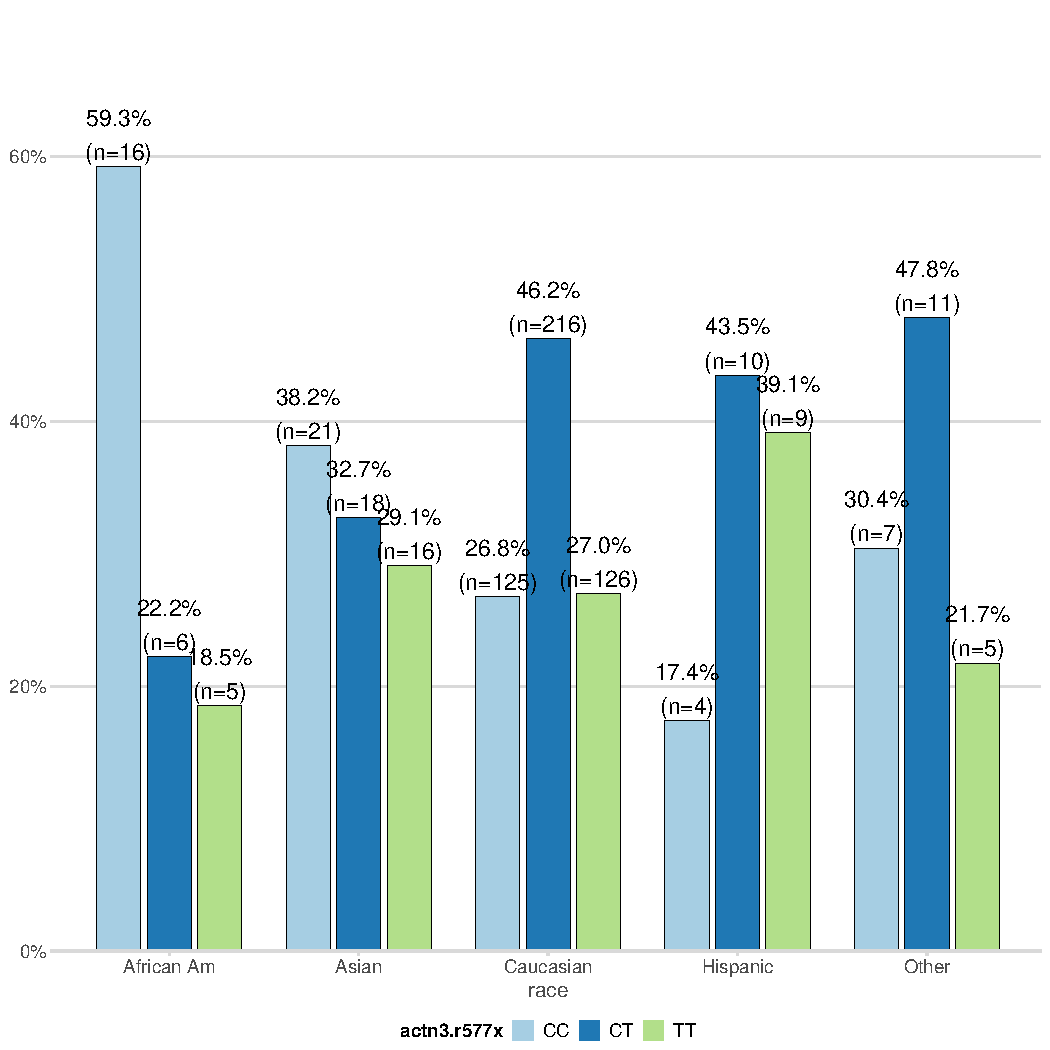
\includegraphics[width=\maxwidth]{figure/genotype-marginals-1} 

}



\end{knitrout}
\end{minipage}
\end{figure}
\end{frame}
	
\begin{frame}[fragile]{Conditional distribution of race \textit{given} genotype}

\begin{knitrout}\tiny
\definecolor{shadecolor}{rgb}{0.969, 0.969, 0.969}\color{fgcolor}\begin{kframe}
\begin{alltt}
\hlkwd{addmargins}\hlstd{(}\hlkwd{prop.table}\hlstd{(tab1,} \hlkwc{margin} \hlstd{=} \hlnum{2}\hlstd{))}
\end{alltt}
\begin{verbatim}
##             
##                 CC    CT    TT   Sum
##   African Am 0.092 0.023 0.031 0.147
##   Asian      0.121 0.069 0.099 0.290
##   Caucasian  0.723 0.828 0.783 2.333
##   Hispanic   0.023 0.038 0.056 0.117
##   Other      0.040 0.042 0.031 0.114
##   Sum        1.000 1.000 1.000 3.000
\end{verbatim}
\end{kframe}
\end{knitrout}

\begin{knitrout}\tiny
\definecolor{shadecolor}{rgb}{0.969, 0.969, 0.969}\color{fgcolor}\begin{kframe}
\begin{alltt}
\hlstd{sjPlot}\hlopt{::}\hlkwd{plot_xtab}\hlstd{(famuss}\hlopt{$}\hlstd{race, famuss}\hlopt{$}\hlstd{actn3.r577x,} \hlkwc{margin} \hlstd{=} \hlstr{"col"}\hlstd{,} \hlkwc{show.total} \hlstd{= F,} \hlkwc{show.n} \hlstd{= F)}
\end{alltt}
\end{kframe}

{\centering 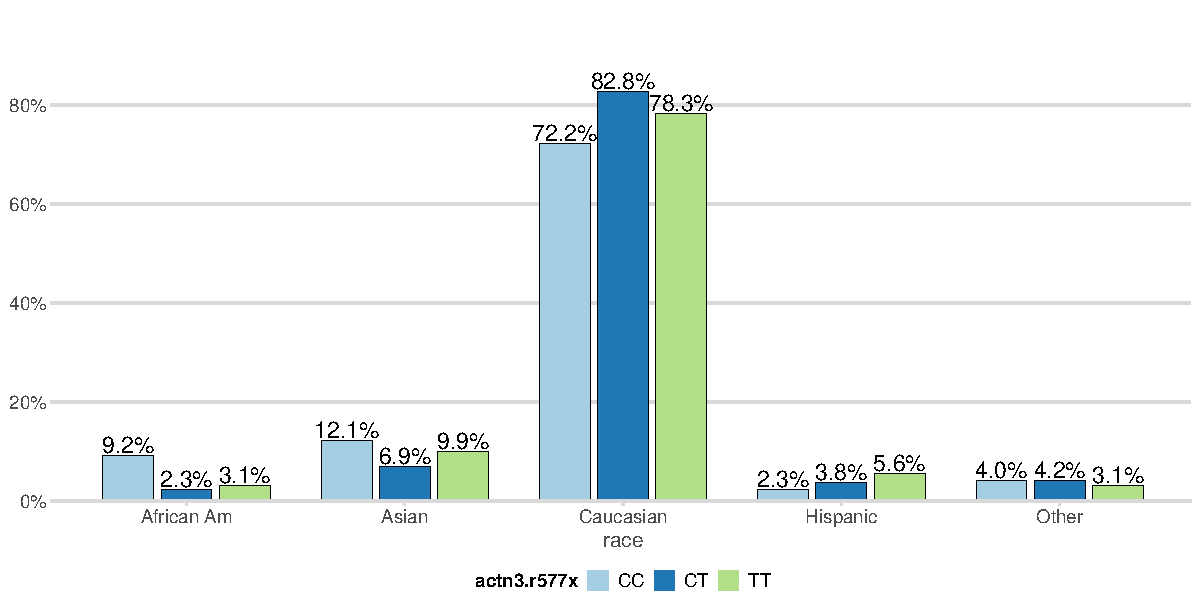
\includegraphics[width=\maxwidth]{figure/race-marginals-1} 

}



\end{knitrout}

\end{frame}

\begin{frame}[fragile]{Marginal distributions of race and genotype}
Given a contingency table, the frequency distribution of one of the variables is called its \textcolor{blue}{\textbf{marginal distribution}}.

\begin{knitrout}\tiny
\definecolor{shadecolor}{rgb}{0.969, 0.969, 0.969}\color{fgcolor}\begin{kframe}
\begin{alltt}
\hlkwd{table}\hlstd{(famuss}\hlopt{$}\hlstd{race)} \hlopt{/} \hlkwd{nrow}\hlstd{(famuss)}
\end{alltt}
\begin{verbatim}
## 
## African Am      Asian  Caucasian   Hispanic      Other 
##      0.045      0.092      0.785      0.039      0.039
\end{verbatim}
\begin{alltt}
\hlstd{sjPlot}\hlopt{::}\hlkwd{plot_frq}\hlstd{(famuss}\hlopt{$}\hlstd{race)}
\hlstd{sjPlot}\hlopt{::}\hlkwd{plot_frq}\hlstd{(famuss}\hlopt{$}\hlstd{actn3.r577x)}
\end{alltt}
\end{kframe}

{\centering 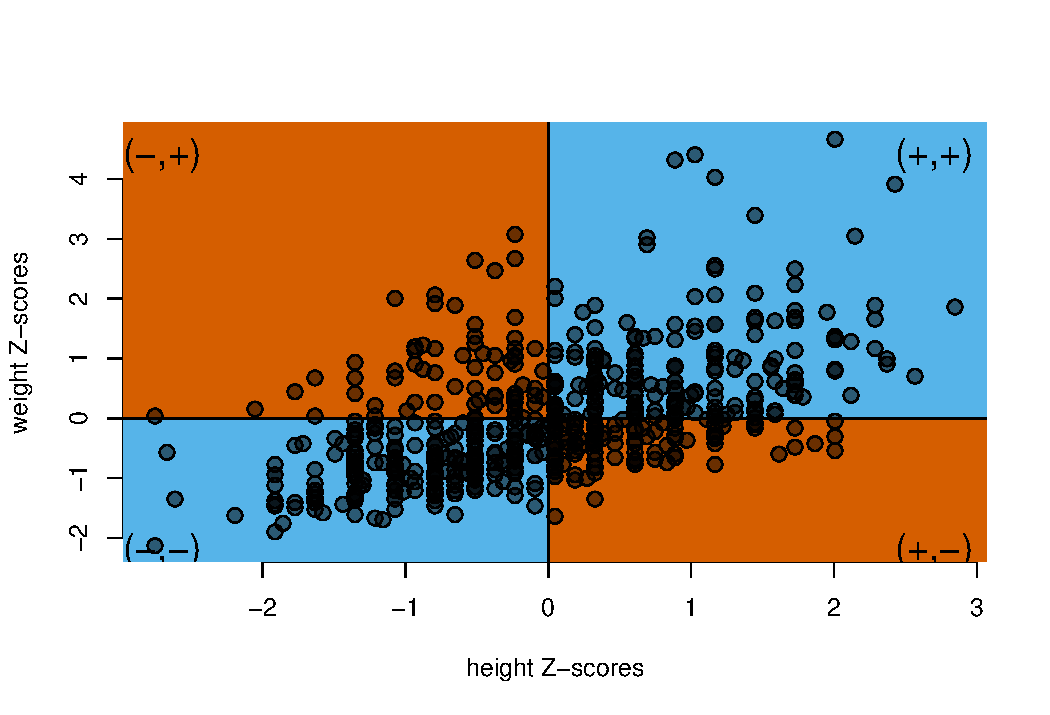
\includegraphics[width=0.45\linewidth]{figure/unnamed-chunk-4-1} 
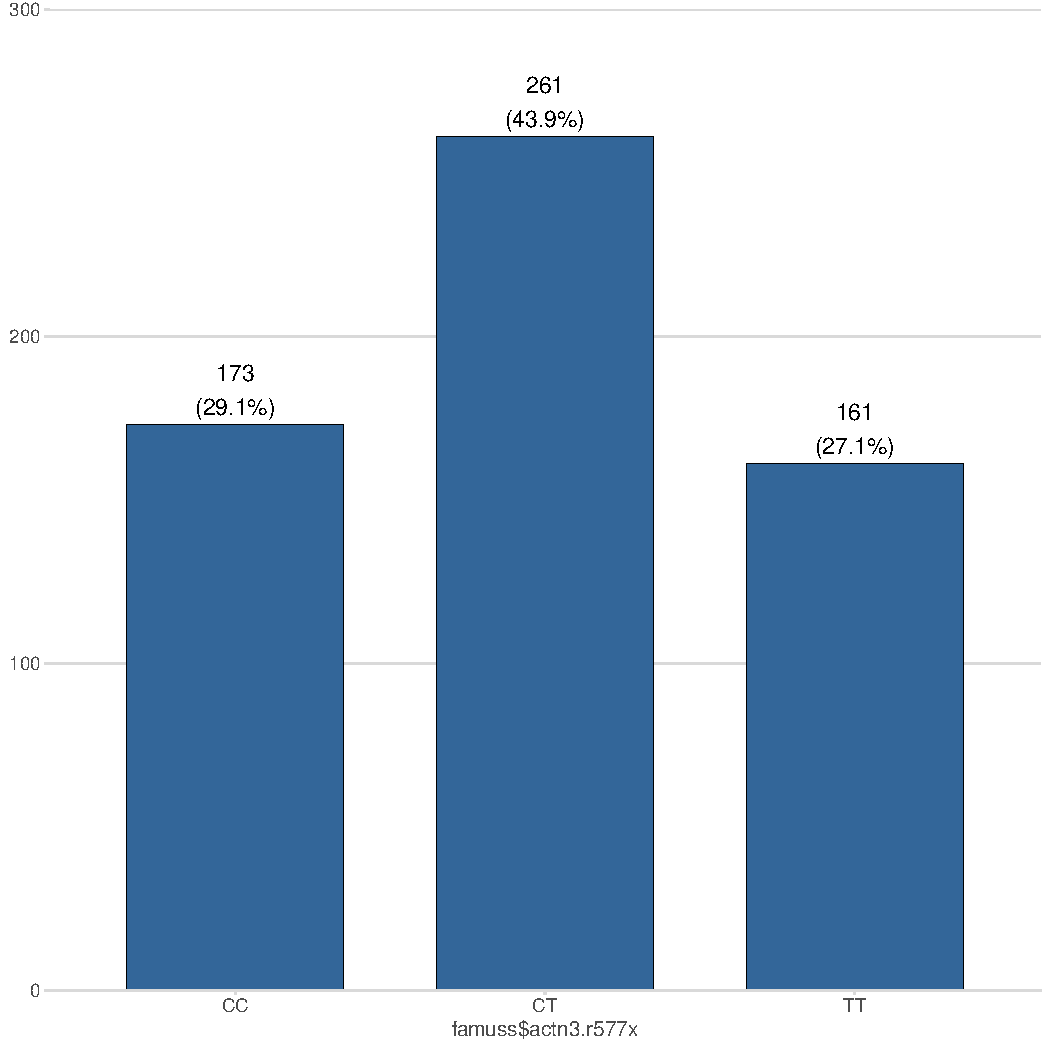
\includegraphics[width=0.45\linewidth]{figure/unnamed-chunk-4-2} 

}



\end{knitrout}

\end{frame}



\begin{frame}{Mosaic plots}
%	\small
\begin{itemize}
	\item A mosaic plot is a graphical display that allows you to examine the relationship among two or more categorical variables.
	\item The mosaic plot starts as a square with length one. The square is divided first into horizontal bars whose widths are proportional to the probabilities associated with the first categorical variable. 
	\item Then each bar is split vertically into bars that are proportional to the conditional probabilities of the second categorical
	variable. Additional splits can be made if wanted using a third, fourth variable, etc.
\end{itemize}

\end{frame}

\begin{frame}[fragile]{Mosaic plots - race and genotype}
	

	
\begin{knitrout}\tiny
\definecolor{shadecolor}{rgb}{0.969, 0.969, 0.969}\color{fgcolor}\begin{kframe}
\begin{alltt}
\hlcom{# devtools::install_github("haleyjeppson/ggmosaic")}
\hlstd{pacman}\hlopt{::}\hlkwd{p_load}\hlstd{(ggmosaic)}
\hlkwd{ggplot}\hlstd{(}\hlkwc{data} \hlstd{= famuss)} \hlopt{+}
  \hlkwd{geom_mosaic}\hlstd{(}\hlkwd{aes}\hlstd{(}\hlkwc{x} \hlstd{=} \hlkwd{product}\hlstd{(race, actn3.r577x),}
                  \hlkwc{fill} \hlstd{= race))}
\end{alltt}
\end{kframe}

{\centering 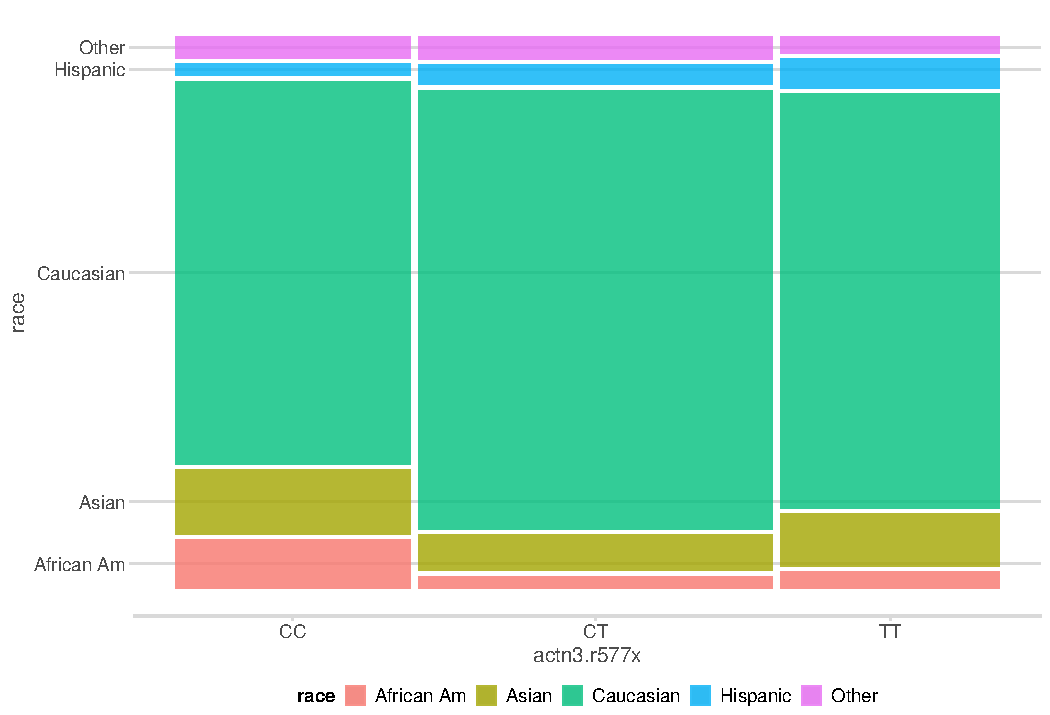
\includegraphics[width=\maxwidth]{figure/mosaic-1-1} 

}



\end{knitrout}
	
\end{frame}



\begin{frame}[fragile]{Mosaic plots - race, genotype and sex}
\begin{knitrout}\tiny
\definecolor{shadecolor}{rgb}{0.969, 0.969, 0.969}\color{fgcolor}\begin{kframe}
\begin{alltt}
    \hlkwd{ggplot}\hlstd{(}\hlkwc{data} \hlstd{= famuss)} \hlopt{+}
      \hlkwd{geom_mosaic}\hlstd{(}\hlkwd{aes}\hlstd{(}\hlkwc{x} \hlstd{=} \hlkwd{product}\hlstd{(race, actn3.r577x),}
                      \hlkwc{fill} \hlstd{= race,} \hlkwc{conds} \hlstd{=} \hlkwd{product}\hlstd{(sex)),}
                      \hlkwc{divider} \hlstd{=} \hlkwd{mosaic}\hlstd{(}\hlstr{"v"}\hlstd{))}
\end{alltt}
\end{kframe}

{\centering 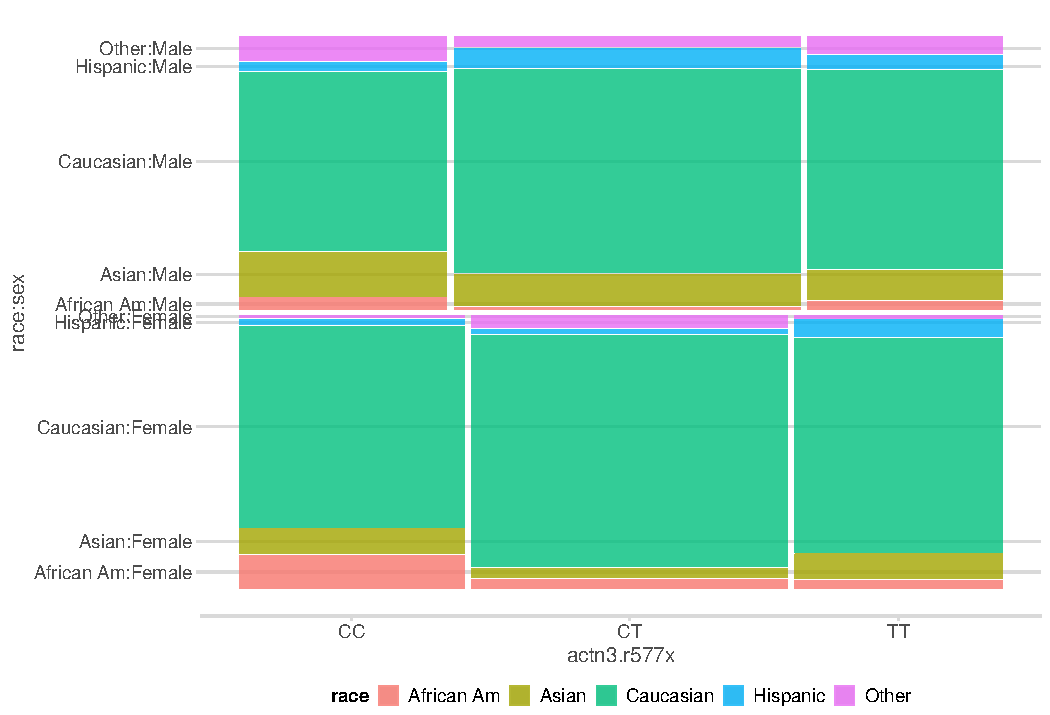
\includegraphics[width=\maxwidth]{figure/mosaic-2-1} 

}



\end{knitrout}
	
\end{frame}



\section{A numerical variable and a categorical variable}

\begin{frame}{A numerical variable and a categorical variable}
	\protect\hypertarget{a-numerical-variable-and-a-categorical-variable}{}
	
	\begin{itemize}
		\item \emph{FAMuSS} was designed to study the relationship between genotype at
	the location \emph{r577x} in the gene \emph{ACTN3} and muscle strength.
	
	\item Muscle strength was assessed by the percent change in non-dominant arm
	strength after resistance training (\texttt{ndrm.ch}).
	
	\item What visualization would be a good choice to make this comparison?
	\end{itemize}
	
\end{frame}


\begin{frame}[fragile]{A numerical variable and a categorical variable}
	\protect\hypertarget{a-numerical-variable-and-a-categorical-variable-1}{}
	
	\scriptsize
	
	\scriptsize
	

	
\begin{knitrout}\scriptsize
\definecolor{shadecolor}{rgb}{0.969, 0.969, 0.969}\color{fgcolor}\begin{kframe}
\begin{alltt}
\hlkwd{ggplot}\hlstd{(}\hlkwc{data} \hlstd{= famuss,} \hlkwc{mapping} \hlstd{=} \hlkwd{aes}\hlstd{(}\hlkwc{x} \hlstd{= actn3.r577x,} \hlkwc{y} \hlstd{= ndrm.ch,} \hlkwc{fill} \hlstd{= actn3.r577x))} \hlopt{+}
  \hlkwd{geom_boxplot}\hlstd{()}
\end{alltt}
\end{kframe}

{\centering 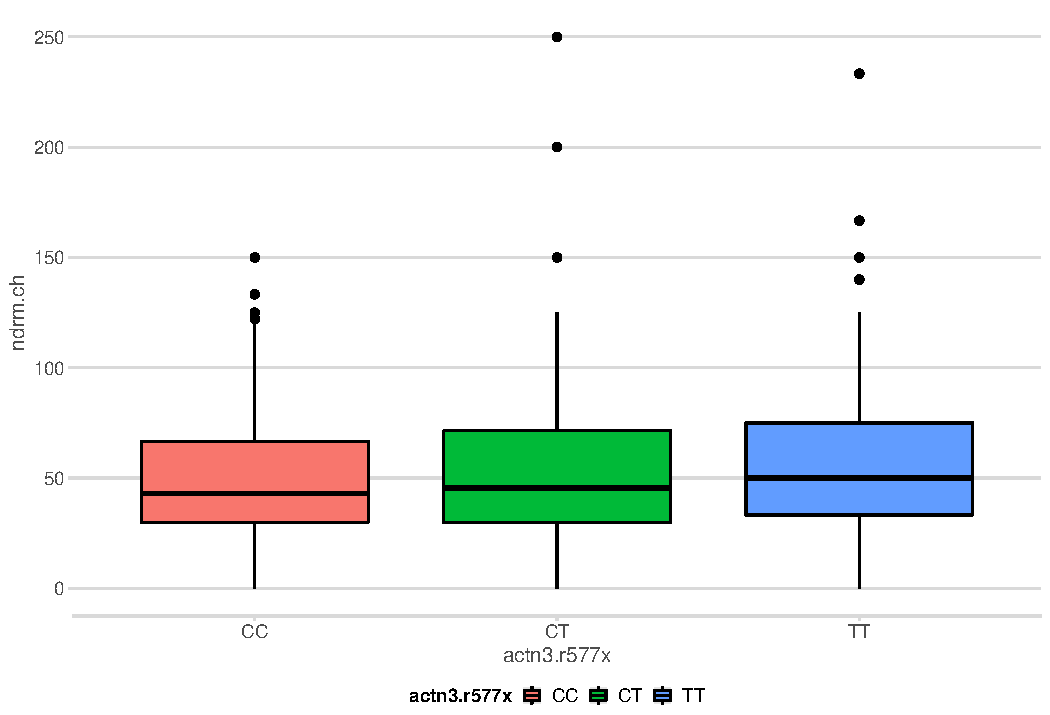
\includegraphics[width=\maxwidth]{figure/box-1-1} 

}



\end{knitrout}
	
	
	\normalsize
	
\end{frame}

\section{Summary}

\begin{frame}{Summary of exploring data slides} 
	
\begin{itemize}
	\item Two types of variables:
	\begin{itemize}
		\item \textbf{Numeric}: Discrete, Continuous
		\item \textbf{Categorical}: Ordinal, Nominal
	\end{itemize}
\pause
\item The collection of values for a numerical or categorical is called the distribution of that variable
\pause
\item Measures of center include mean and median. 
\item Measures of spread include standard deviation, interquartile range
\item Median and IQR are robust to outliers
\pause
\item Histograms, boxplots, violin plots, and scatterplots are useful graphical summaries of numerical data, which can also be grouped by a categorical variable
\item Bar plots, contingency tables, mosaic plots are useful summaries of categorical data
\end{itemize}
\end{frame}

\begin{frame}{Summary of exploring data slides \textit{continued}} 
	
	\begin{itemize}
		\item Correlation coefficient ($r$) quantifies the strength of a linear trend. 
		\item The \texttt{multiple R-squared} in a simple linear regression output is equal to $r^2$. 
		\item Transformation (e.g. log) can produce better linear associations for highly skewed data. But be careful about the interpretation!
		\pause
		\item Given a contingency table, the frequency distribution of one of the variables is called its marginal distribution
		\item Conditional distributions show the distribution of one variable for just those cases that satisfy a condition on another variable
		\item See \url{https://www.r-graph-gallery.com/} and \url{https://www.data-to-viz.com/} for a collection of graphical displays
	\end{itemize}
\end{frame}

\begin{frame}[fragile]{Session Info}
	\tiny
	
\begin{knitrout}\tiny
\definecolor{shadecolor}{rgb}{0.969, 0.969, 0.969}\color{fgcolor}\begin{kframe}
\begin{verbatim}
R version 3.6.2 (2019-12-12)
Platform: x86_64-pc-linux-gnu (64-bit)
Running under: Pop!_OS 19.10

Matrix products: default
BLAS:   /usr/lib/x86_64-linux-gnu/openblas/libblas.so.3
LAPACK: /usr/lib/x86_64-linux-gnu/libopenblasp-r0.3.7.so

attached base packages:
[1] tools     stats     graphics  grDevices utils     datasets  methods  
[8] base     

other attached packages:
 [1] ggmosaic_0.3.0      cowplot_1.0.0       openintro_2.0.0    
 [4] usdata_0.1.0        cherryblossom_0.1.0 airports_0.1.0     
 [7] oibiostat_0.2.0     NCStats_0.4.7       FSA_0.8.30         
[10] forcats_0.5.0       stringr_1.4.0       dplyr_1.0.2        
[13] purrr_0.3.4         readr_1.3.1         tidyr_1.1.2        
[16] tibble_3.0.3        ggplot2_3.3.2.9000  tidyverse_1.3.0    
[19] knitr_1.29         

loaded via a namespace (and not attached):
 [1] nlme_3.1-143       fs_1.3.2           lubridate_1.7.4    RColorBrewer_1.1-2
 [5] insight_0.8.1      httr_1.4.1         backports_1.1.9    R6_2.4.1          
 [9] sjlabelled_1.1.3   lazyeval_0.2.2     DBI_1.1.0          colorspace_1.4-1  
[13] withr_2.2.0        tidyselect_1.1.0   emmeans_1.4.5      compiler_3.6.2    
[17] performance_0.4.4  cli_2.0.2          rvest_0.3.5        pacman_0.5.1      
[21] xml2_1.3.0         plotly_4.9.2       sandwich_2.5-1     labeling_0.3      
[25] bayestestR_0.5.2   scales_1.1.1       mvtnorm_1.0-12     digest_0.6.25     
[29] minqa_1.2.4        htmltools_0.5.0    pkgconfig_2.0.3    lme4_1.1-21       
[33] dbplyr_1.4.2       highr_0.8          htmlwidgets_1.5.1  rlang_0.4.7       
[37] readxl_1.3.1       rstudioapi_0.11    farver_2.0.3       generics_0.0.2    
[41] zoo_1.8-7          jsonlite_1.7.0     sjPlot_2.8.3       magrittr_1.5      
[45] parameters_0.5.0   Matrix_1.2-18      Rcpp_1.0.4.6       munsell_0.5.0     
[49] fansi_0.4.1        lifecycle_0.2.0    stringi_1.4.6      multcomp_1.4-12   
[53] snakecase_0.11.0   MASS_7.3-51.5      plyr_1.8.6         grid_3.6.2        
[57] sjmisc_2.8.3       crayon_1.3.4       lattice_0.20-38    ggeffects_0.14.1  
[61] haven_2.3.1        splines_3.6.2      sjstats_0.17.9     hms_0.5.3         
[65] pillar_1.4.6       boot_1.3-24        estimability_1.3   effectsize_0.2.0  
[69] codetools_0.2-16   reprex_0.3.0       glue_1.4.2         evaluate_0.14     
[73] data.table_1.12.8  modelr_0.1.5       vctrs_0.3.4        nloptr_1.2.2.1    
[77] cellranger_1.1.0   gtable_0.3.0       productplots_0.1.1 assertthat_0.2.1  
[81] TeachingDemos_2.12 xfun_0.16          xtable_1.8-4       broom_0.7.0       
[85] coda_0.19-3        viridisLite_0.3.0  survival_3.1-8     TH.data_1.0-10    
[89] ellipsis_0.3.1    
\end{verbatim}
\end{kframe}
\end{knitrout}
	
\end{frame}

\end{document}	
	
\hypertarget{case-study-molecular-cancer-classification}{%
\section{Case study: molecular cancer classification}\label{case-study-molecular-cancer-classification}}
						
\begin{frame}{The potential value of genomic data in cancer}
							\protect\hypertarget{the-potential-value-of-genomic-data-in-cancer}{}
							
							The majority of cancers are diagnosed by an expert pathologist examining
							slides of malignant cells.
							
							Can that be done more accurately by characterizing the genetic makeup of
							the malignancy?
							
							\begin{itemize}
								\tightlist
								\item
								This is perhaps the major potential of genomic characterizations of
								tumors.
							\end{itemize}
							
							There are many forms of childhood leukemia.
							
							\begin{itemize}
								\item
								Acute myeloblastic leukemia (AML) and acute lymphoblastic leukemia
								(ALL) are the most common.
								\item
								AML is a cancer of the bone marrow, where white blood cells
								(lymphocytes) are produced.
								\item
								ALL is a cancer of the lymphocytes and is designated as B-cell (ALLB)
								or T-cell (ALLT).
							\end{itemize}
							
\end{frame}


		
\begin{frame}{Prognosis of the two cancers}
							\protect\hypertarget{prognosis-of-the-two-cancers}{}
							
							The probability that a child diagnosed with ALL is survives at least 5
							years after the diagnosis is approximately 90\%.
							
							Approximately 65\% of children diagnosed with AML survive at least 5
							years.
							
							The diagnosis of leukemia type determines the therapy that will be given
							to the child, and the successful treatments for ALL and AML are
							different.
							
							In 1999, Todd Golub from the Dana-Farber and the Broad Institute
							examined the possibility of classifying leukemia through using a genetic
							analysis of a blood sample.
							
						\end{frame}
						
						\begin{frame}{Analyzing the Golub data}
							\protect\hypertarget{analyzing-the-golub-data}{}
							
							We can re-analyze the Golub data using tools from graphical and
							numerical summaries.
							
							Our analysis will not be identical to the Golub analysis, but will be
							similar in spirit.
							
							The tools are straighforward\ldots   
							
							\begin{itemize}
								\item
								Thinking through the problem and assembling the tools is the hard
								part.
								\item
								The process is more important than the final recipe.
							\end{itemize}
							
						\end{frame}
						
						\begin{frame}{Gene expression (details in \emph{OI Biostat})}
							\protect\hypertarget{gene-expression-details-in-oi-biostat}{}
							
							\small
							
							\begin{itemize}
								\item
								The genetic code stored in DNA contains the information for producing
								the proteins that determine an organism's phenotype.
								\item
								Genes that are transcriptionally active (i.e.~turned ``on'') are
								transcribed into messenger RNA (mRNA) that gets translated into
								proteins.
								\item
								Genes can be switched on or off, and expressed at varying levels.
								Variations in gene expression produce the range of physical,
								biochemical, and developmental differences in cells and tissues.
								\item
								Quantifying the amount of RNA produced in a cell allows for a measure
								of gene expression.
								\item
								The transcriptome, or expression profile, is the complete set of RNA
								transcripts produced by the genome in a cell or set of cells.
							\end{itemize}
							
						\end{frame}
						
						\begin{frame}{Microarrays (details in \emph{OI Biostat})}
							\protect\hypertarget{microarrays-details-in-oi-biostat}{}
							
							\small
							
							\begin{itemize}
								\item
								Microarray technology is based on hybridization between two DNA
								strands, in which complementary nucleotide sequences specifically pair
								together.
								\item
								The mRNA from a sample is converted into complementary-DNA (cDNA),
								labeled with a fluorescent dye, and added to the microarray.
								\item
								When cDNA from the sample encounters complementary DNA probes, the two
								strands will hybridize, allowing the cDNA to adhere to specific spots
								on the slide.
								\item
								When the chip is illuminated and scanned, the intensity of
								fluorescence detected at each spot corresponds to the amount of bound
								cDNA.
								\item
								DNA microarrays do not directly quantify gene expression levels or
								quantity of mRNA present in a sample.
								\item
								The fluorescence intensity data only provide a relative measure of
								gene expression, showing which genes on the chip seem to be more or
								less active in relation to each other.
							\end{itemize}
							
						\end{frame}
						
						\begin{frame}{Microarrays}
							\protect\hypertarget{microarrays}{}
							
							\begin{figure}
								\centering
								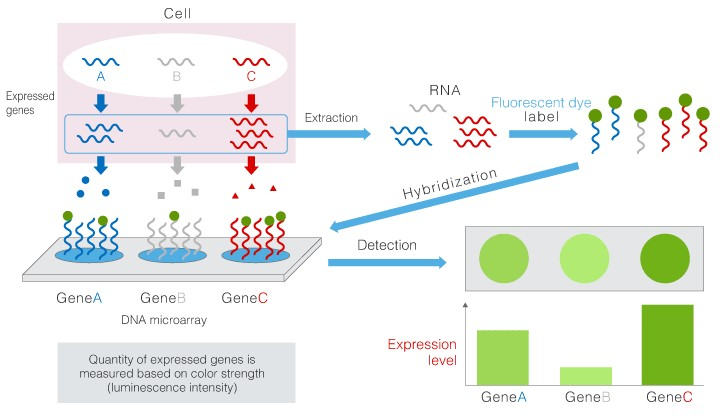
\includegraphics[scale=0.5]{figures/microarray_schematic.jpg}
								\caption{fluorescence detection}
							\end{figure}
							
						\end{frame}
						
						\begin{frame}{The Golub clinical data}
							\protect\hypertarget{the-golub-clinical-data}{}
							
							Demographic variables described in \emph{OI Biostat} Table 1.54:
							
							\scriptsize
							
							\begin{longtable}[]{@{}ll@{}}
								\toprule
								\begin{minipage}[b]{0.12\columnwidth}\raggedright
									Variable\strut
								\end{minipage} & \begin{minipage}[b]{0.82\columnwidth}\raggedright
									Description\strut
								\end{minipage}\tabularnewline
								\midrule
								\endhead
								\begin{minipage}[t]{0.12\columnwidth}\raggedright
									Samples\strut
								\end{minipage} & \begin{minipage}[t]{0.82\columnwidth}\raggedright
									Sample or chip number. The material from each patient was examined on a
									separate chip and experimental run.\strut
								\end{minipage}\tabularnewline
								\begin{minipage}[t]{0.12\columnwidth}\raggedright
									BM.PB\strut
								\end{minipage} & \begin{minipage}[t]{0.82\columnwidth}\raggedright
									Type of patient material. BM denotes bone marrow; PB denotes a
									peripheral blood sample.\strut
								\end{minipage}\tabularnewline
								\begin{minipage}[t]{0.12\columnwidth}\raggedright
									Gender\strut
								\end{minipage} & \begin{minipage}[t]{0.82\columnwidth}\raggedright
									F for female, M for male.\strut
								\end{minipage}\tabularnewline
								\begin{minipage}[t]{0.12\columnwidth}\raggedright
									Source\strut
								\end{minipage} & \begin{minipage}[t]{0.82\columnwidth}\raggedright
									Hospital where the patient was treated.\strut
								\end{minipage}\tabularnewline
								\begin{minipage}[t]{0.12\columnwidth}\raggedright
									tissue.mf\strut
								\end{minipage} & \begin{minipage}[t]{0.82\columnwidth}\raggedright
									A variable showing the combination of type of patient material and sex
									of the patient. BM:f denotes bone marrow from a female patient,
									etc.\strut
								\end{minipage}\tabularnewline
								\begin{minipage}[t]{0.12\columnwidth}\raggedright
									cancer\strut
								\end{minipage} & \begin{minipage}[t]{0.82\columnwidth}\raggedright
									The type of leukemia; aml is acute myeloblastic leukemia, allB is acute
									lymphoblastic leukemia which started in B-cells (cells that mature into
									plasma cells) origin, and allT is acute lymphoblastic leukemia with
									T-cell origin (T-cells are a type of white blood cell).\strut
								\end{minipage}\tabularnewline
								\bottomrule
							\end{longtable}
							
						\end{frame}
						
						\begin{frame}{The Golub expression data}
							\protect\hypertarget{the-golub-expression-data}{}
							
							The expression data is contained in the last 7,129 columns.
							
							Each column is a variable with a name corresponding to the name of the
							probe on the microarray.
							
							The expression levels record fluorescence intensity for each gene.
							
							\begin{itemize}
								\item
								The intensity levels have no inherent biological meaning.
								\item
								Data have been normalized to adjust for variability between the
								separate arrays used for each patient.
							\end{itemize}
							
						\end{frame}
						
						\begin{frame}{Selected variables and columns from Golub data}
							\protect\hypertarget{selected-variables-and-columns-from-golub-data}{}
							
							\captionsetup[table]{labelformat=empty}
							\scriptsize
							
							\scriptsize
							
							\begin{longtable}[]{@{}rllrrr@{}}
								\caption{\emph{OI Biostat} Table 1.40}\tabularnewline
								\toprule
								Samples & Gender & cancer & AFFX-BioB-5\_at & AFFX-BioB-M\_at &
								AFFX-BioB-3\_at\tabularnewline
								\midrule
								\endfirsthead
								\toprule
								Samples & Gender & cancer & AFFX-BioB-5\_at & AFFX-BioB-M\_at &
								AFFX-BioB-3\_at\tabularnewline
								\midrule
								\endhead
								39 & F & allB & -1363.28 & -1058.59 & -541.47\tabularnewline
								40 & F & allB & -796.29 & -1167.10 & 7.54\tabularnewline
								42 & F & allB & -679.14 & -1069.83 & -690.30\tabularnewline
								47 & M & allB & -1164.40 & -1109.94 & -990.13\tabularnewline
								48 & F & allB & -1299.65 & -1402.00 & -1077.54\tabularnewline
								\bottomrule
							\end{longtable}
							
							\normalsize
							
						\end{frame}
						
						\begin{frame}{Analyzing the Golub leukemia data}
							\protect\hypertarget{analyzing-the-golub-leukemia-data}{}
							
							We will do an analysis in class using some of the simple but
							surprisingly powerful ideas behind numerical and graphical summaries.
							
							The goal of the Golub study was to develop a procedure for
							distinguishing between AML and ALL based only on the gene expression
							levels of a patient. There are two major issues to be addressed:
							
							\begin{enumerate}
								\item
								Which genes are the most informative for making a prediction?
								\item
								What is a workable strategy for predicting leukemia type from
								expression data for a specific set of genes?
							\end{enumerate}
							
						\end{frame}
						
						\begin{frame}[fragile]{Starting small\ldots{}}
							\protect\hypertarget{starting-small}{}
							
							\footnotesize
							
							\scriptsize
							
\begin{verbatim}
##    cancer        A         B        C        D
## 69   allB 39307.96 35232.401 41170.76 35792.79
## 67   allT 32281.88 41432.024 59328.51 49608.14
## 55   allB 47429.94 35568.928 56074.96 42857.78
## 56   allB 25533.87 16983.749 28056.75 32693.92
## 59   allB 35960.55 24191.746 27637.90 22240.75
## 52    aml 46177.95  6189.465 12557.24 34485.41
## 53    aml 43790.70 33661.825 38380.30 29758.25
## 51    aml 53420.05 26109.245 31427.20 23809.70
## 50    aml 41241.59 37589.773 47325.77 30099.36
## 54    aml 41300.57 49198.412 66026.10 56248.62
\end{verbatim}
\end{frame}
						



%\begin{frame}[allowframebreaks]
%\nocite{breiman1984classification}
%	\nocite{friedman2001elements}
%	\nocite{james2013introduction}
%	\nocite{lopez2015arbres}
%	\frametitle{References}
%\printbibliography
%\end{frame}




\end{document}
